%! TEX root = **/010-main.tex
% vim: spell spelllang=en:

\section{Context and scope}%
\label{sec:context}

\subsection{Introduction and contextualization}%
\label{sub:intro}

Since its release in 2007, Compute Unified Device Architecture (CUDA) has
revolutionized the usage of graphic processing units for scientific
computations, allowing developers to implement programs that take full advantage
of the parallelization capabilities of GPUs for general purpose programming.
This paired with the exponential growth of computing power that GPUs have
experienced in the last decade has made GPU numerical analysis essential on
modern science research. Highly complex problems that where once impossible to
compute in realistic time frames can now be computed even on average consumer
hardware GPUs. Moreover, projects like
\emph{GPUGRID}\footnote{\url{www.gpugrid.net}} allow researches to run
distributed programs through a grid of GPUs from volunteers all over the world
reaching supercomputing level performance \cite{antaviana_nvidia_nodate}.


In 1900 David Hilbert posed a list of 23 problems in the field of mathematics
which were unsolved at the time \cite{hilbert_mathematische_1900}.  Those
problems have been vastly studied since then and most of them are solved or
partially solved. There are however some which are still unsolved to this day.

One of these unsolved problems is the 16th problem.  This problem consists of
two separate problems, the first one regarding the relative positions of the
branches of real algebraic curves and the second one about the upper limit of
limit cycles on two dimensional vector fields and their relative positions. In
this project we are going to study the second part of this 16th problem.

In particular, we study the number of limit cycles for vector fields of
polynomials of second degree:
\begin{align}
    \frac{dx}{dt} &= a_1x^2 + b_1xy + c_1y^2 + \alpha_1x + \beta_1y \\
    \frac{dy}{dt} &= a_2x^2 + b_2xy + c_2y^2 + \alpha_2x + \beta_2y
\end{align}

It is unknown whether there exists an upper limit on the number of limit cycles for systems with polynomials of degree greater than one\cite{ilyashenko_centennial_2002}. 
For a moment, the largest number of limit cycles is equal to four and it is an open question if a larger number of limit cycles is possible.
% todo
% Determining if a point is part of a limit cycle is shown to be
% \textbf{PSPACE}-complete  \cite{papadimitriou_computational_2015}

\subsubsection{Context}

This is a Bachelor Thesis of the Computer Engineering Degree, specialization in
Computing, done in the Facultat Inform\`atica de Barcelona (FIB) of the
Universitat Polit\'ecnica de Catalunya (UPC). The project is directed by Grigori
Astrakharchik.

\subsubsection{Concepts}

Below are some concepts needed to understand the project.

\newcommand{\concept}[1]{\textbf{#1}\\}

% \concept{Ordinary differential equations}
%todo

\concept{Limit cycles}
A limit cycle is a closed trajectory with the property that at least one other
trajectory spirals into it as time approaches infinity. They are important in
various applications in the field of dynamical systems.

\concept{CUDA}
CUDA is a parallel computing platform developed by \emph{nvidia} that allows general
computing on their graphic processing units (GPUs). Using the CUDA programming
model allows developers to run massively parallel programs on GPUs.

\subsubsection{Problem to be solved}

There have been various studies on the number of limit cycles for second degree vector fields but so far the maximum number of cycles found is 4, as shown in Ref.~\cite{kuznetsov_visualization_2013}. The aim of this project is to search the
parameter space for systems that have 4 or more cycles to gain more insight on
the nature of these equations.

\Cref{fig:kuznetsov} shows a characteristic example of a visualization of the limit cycles in a two-dimensional polynomial quadratic system.

\begin{figure}[H]
    \centering
    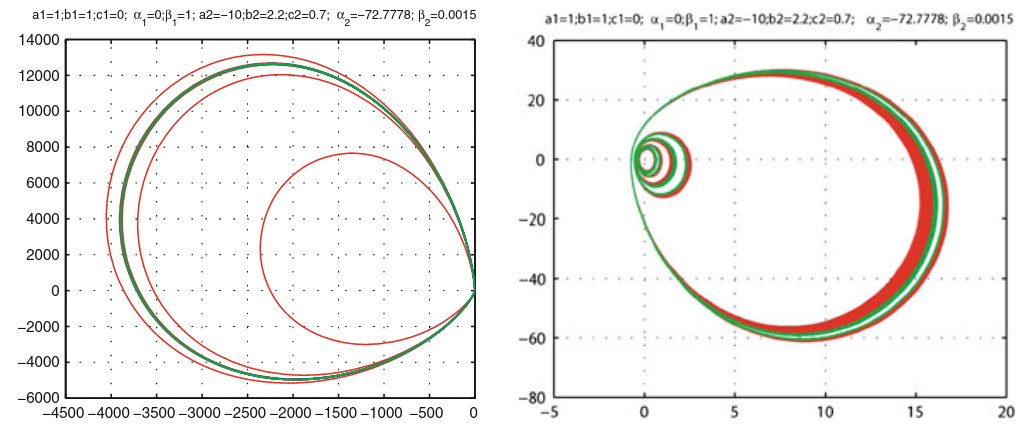
\includegraphics[width=1.0\textwidth]{4cycles}
    \caption{Visualization of four limit cycles in two-dimensional polynomial quadratic system, from Ref.~\cite{kuznetsov_visualization_2013}
    }%
    \label{fig:kuznetsov}
\end{figure}

To do so, we will implement an efficient parallel algorithm that solves systems of ordinary differential equations (ODE) and
detects limit cycles for a wide range of parameters and points in the plane.
This code will be implemented in Julia programming language and will use CUDA framework
in such a way that massive parallel calculation can be done on a dedicated CUDA server with several advanced GPU graphic cards.

%\subsubsection{Stakeholders}

\subsection{Justification}
\subsubsection{Previous studies}

There have been a number of studies relying on numerical methods to find limit cycles in
two dimensional vector fields
\cite{leonov_hidden_2013,van_der_hoff_numerical_2013,casades_computation_2013,gasull_effective_nodate}.
Papadimitriou and Vishnoi showed that the computation of a limit cycle is
% PSPACE??
\textbf{PSPACE}-complete~\cite{papadimitriou_computational_2015}.
The maximal known number of limit cycles is reported in Kuznetsov et al.~\cite{kuznetsov_visualization_2013} where an example of specific conditions for which 4 limit cycles is provided.

% todo

There are various programming languages (C, C++, Fortran, Python and MATLAB) compatible with CUDA and which have libraries for CUDA programming. 
%There are various programming languages with libraries for CUDA programming.
%In GPU-accelerated applications, the sequential part of the workload runs on the CPU – which is optimized for single-threaded performance – while the compute intensive portion of the application runs on thousands of GPU cores in parallel. When using CUDA, developers program in popular languages such as C, C++, Fortran, Python and MATLAB and express parallelism through extensions in the form of a few basic keywords.
The official CUDA programming model is in C/C++ and offers the most flexibility and performance. The other two most notable alternatives are Python's Numba and Julia's CUDA.jl. 
These are higher-level libraries and 
are more limited in the versatility 
%do not offer the same low level options 
but allow easier development and visualization of the data.
Both Python and Julia use the official CUDA C interface under the hood so although the performance is not as good as with pure C, if an appropriate realization of the methods is done, the performance might be still good if the majority of the work is done in the CUDA kernels. Since Julia JIT compilation is faster than the python's one and provides similar advantages when visualizing data the initial idea is to program the whole project in Julia programming language.

This is not a strict constraint and the possibility of writing specific C CUDA code to tweak the performance to the maximum will be studied.

% todo

\subsection{Scope}
\subsubsection{Objectives and sub-objectives}

The main objective of this Thesis is to develop a highly-efficient code capable of determining the possible existence of limit cycles for a system. This code must also be capable of being executed in parallel in a GPU cluster making full use of its computing power to simulate a wide variety of systems with different parameters. Furthermore the results must be processed to find interesting
systems to visualize and analyse in more detail. These objectives can be divided in sub-objectives:

\paragraph{Theoretical part} 

Before implementing the algorithms and developing the code, a deep understanding of the current numerical methods and the CUDA framework must be achieved to find the best approach to the problem.

\begin{itemize}
    \item Explore the best strategies to solve ordinary differential equations.
    \item Explore numerical methods to verify the existence of limit cycles and determine the number of cycles for a given system.
    \item Research how these methods can be applied to run in a CUDA system efficiently.
\end{itemize}

\paragraph{Practical part} Having done the background research, the code must be developed, implemented and tested. 
Different methods will be tried in order to find the ones that give the best performance.

\begin{itemize}
    \item Implement the algorithms in an efficient code.
    \item Benchmark the performance and compare different approaches to achieve the best performance.
    \item Run the code on a dedicated GPU server.
    \item Analyze the results and visualize them.
    \item Present and discuss the obtained results in the Thesis.
\end{itemize}

\subsubsection{Requirements}

To ensure the quality of the Thesis a number of requirements must be fulfilled:
\begin{itemize}
    \item Find the best balance between accuracy of the results and computational complexity
    \item Ensure that the numerical methods applied are properly implemented.
    \item Take into account numerical stability of the methods used as well as rounding and overflow errors.
    \item Profile the different methods under the same conditions and environment to ensure that there are no biases.
    \item Use good programming practices, making readable and maintainable code with the least complexity possible.
    \item Make the developed code publicly available.
\end{itemize}

\subsubsection{Potential obstacles and risks}

There are several risks that may have to be dealt with during the development of this thesis.

\begin{itemize}
    \item \textbf{Project deadlines}: There is a limited amount of time to do the project. Therefore a proper planning of tasks and time must be made and followed to ensure that the work can be done in the proper time frame.
    \item \textbf{Computational power}: This Thesis involves a lot of computational power and the whole project is conditioned by it. If the program cannot be run on the proper hardware the results may not be obtainable in a realistic time frame and the scope of the project will have to be reevaluated.
    \item \textbf{Inexperience on the field}: I have very limited experience with CUDA programming and just the basics of numerical computation techniques so there is a lot of research to be done, specially regarding      dynamical systems.
\end{itemize}

\subsection{Methodology and rigor}

\subsubsection{Methodology}

Since the Thesis must be completed in a relatively short period of time we will apply the \emph{agile} methodology and divide the work into sub-tasks or \emph{sprints}. These \emph{sprints} will consist of different stages of  implementation of the program, beginning with a proof of concept running in sequence on the CPU and progressively iterating on this base to optimize the methods and adapt them to be able to run in CUDA on the GPU.

\subsubsection{Monitoring tools and validation}

To manage the different iterations of the code \texttt{git} will be used. The repository will be hosted on \emph{GitHub} and access will be granted to the project tutor allowing him to follow and monitor the work and results at any time.

A weekly meeting with the tutor will be arranged to discuss the progress and which tasks should be worked on.